% Options for packages loaded elsewhere
\PassOptionsToPackage{unicode}{hyperref}
\PassOptionsToPackage{hyphens}{url}
%
\documentclass[
]{article}
\usepackage{amsmath,amssymb}
\usepackage{iftex}
\ifPDFTeX
  \usepackage[T1]{fontenc}
  \usepackage[utf8]{inputenc}
  \usepackage{textcomp} % provide euro and other symbols
\else % if luatex or xetex
  \usepackage{unicode-math} % this also loads fontspec
  \defaultfontfeatures{Scale=MatchLowercase}
  \defaultfontfeatures[\rmfamily]{Ligatures=TeX,Scale=1}
\fi
\usepackage{lmodern}
\ifPDFTeX\else
  % xetex/luatex font selection
\fi
% Use upquote if available, for straight quotes in verbatim environments
\IfFileExists{upquote.sty}{\usepackage{upquote}}{}
\IfFileExists{microtype.sty}{% use microtype if available
  \usepackage[]{microtype}
  \UseMicrotypeSet[protrusion]{basicmath} % disable protrusion for tt fonts
}{}
\makeatletter
\@ifundefined{KOMAClassName}{% if non-KOMA class
  \IfFileExists{parskip.sty}{%
    \usepackage{parskip}
  }{% else
    \setlength{\parindent}{0pt}
    \setlength{\parskip}{6pt plus 2pt minus 1pt}}
}{% if KOMA class
  \KOMAoptions{parskip=half}}
\makeatother
\usepackage{xcolor}
\usepackage[margin=1in]{geometry}
\usepackage{longtable,booktabs,array}
\usepackage{calc} % for calculating minipage widths
% Correct order of tables after \paragraph or \subparagraph
\usepackage{etoolbox}
\makeatletter
\patchcmd\longtable{\par}{\if@noskipsec\mbox{}\fi\par}{}{}
\makeatother
% Allow footnotes in longtable head/foot
\IfFileExists{footnotehyper.sty}{\usepackage{footnotehyper}}{\usepackage{footnote}}
\makesavenoteenv{longtable}
\usepackage{graphicx}
\makeatletter
\def\maxwidth{\ifdim\Gin@nat@width>\linewidth\linewidth\else\Gin@nat@width\fi}
\def\maxheight{\ifdim\Gin@nat@height>\textheight\textheight\else\Gin@nat@height\fi}
\makeatother
% Scale images if necessary, so that they will not overflow the page
% margins by default, and it is still possible to overwrite the defaults
% using explicit options in \includegraphics[width, height, ...]{}
\setkeys{Gin}{width=\maxwidth,height=\maxheight,keepaspectratio}
% Set default figure placement to htbp
\makeatletter
\def\fps@figure{htbp}
\makeatother
\setlength{\emergencystretch}{3em} % prevent overfull lines
\providecommand{\tightlist}{%
  \setlength{\itemsep}{0pt}\setlength{\parskip}{0pt}}
\setcounter{secnumdepth}{-\maxdimen} % remove section numbering
\ifLuaTeX
  \usepackage{selnolig}  % disable illegal ligatures
\fi
\IfFileExists{bookmark.sty}{\usepackage{bookmark}}{\usepackage{hyperref}}
\IfFileExists{xurl.sty}{\usepackage{xurl}}{} % add URL line breaks if available
\urlstyle{same}
\hypersetup{
  pdftitle={Final Exploratory Analysis},
  pdfauthor={Caroline Roeder and Indira Aitkulova},
  hidelinks,
  pdfcreator={LaTeX via pandoc}}

\title{Final Exploratory Analysis}
\author{Caroline Roeder and Indira Aitkulova}
\date{2023-11-27}

\begin{document}
\maketitle

\hypertarget{topic}{%
\subsubsection{Topic}\label{topic}}

What is the relationship between ethanol demand and state-level
legislation?

\hypertarget{motivation}{%
\subsubsection{Motivation}\label{motivation}}

Ethanol is a good source of clean energy. Incorporating it into gasoline
allows for cleaner vehicle fuel sources. Moreover, ethanol is produced
domestically from domestically grown crops, reducing U.S. dependence on
foreign oil and increasing the nation's energy independence. Therefore,
derived from domestically cultivated crops, ethanol not only promotes
environmental responsibility but also strengthens the US nation's energy
independence by reducing dependency on international sources.

Since the 1990s, state and federal governments enacted more than 300
laws incentivizing a market for ethanol. In this study we will
specifically focus on state-level legislation. While federal legislation
is likely related to changes in ethanol demand across all states,
focusing on state-level legislation will allow us to consider how
differential policies to promote ethanol production and use are related
to differential changes in ethanol demand in individual states.

In order to investigate the relationship, we choose the number of E85
stations available as a proxy for ethanol demand. The term E85
specifically denotes a blend containing 85\% ethanol and 15\% gasoline
or other hydrocarbon, measured by volume. This blend represents the
highest ethanol concentration commonly used in vehicles today. Other
fuel blends, E10 and E15, can be run in most engine types. These fuel
blends, requiring smaller shares of ethanol, are commonly required by
legislation whereas E85 is not required. Not all vehicles can use E85
fuel, so consumers purchasing E85 fuel make an active decision to
operate a vehicle which can use E85 and then purchase E85 fuel. For
these reasons, we assume the number of E85 stations approximates ethanol
demand. If legislation increased the number of E85 stations, consumer
demand may have been driven by increased availability. Or, conversely,
consumers with a high demand for E85 fuel may have lobbied for
state-level legislation increasing the number of E85 stations.
Therefore, this project aims to investigate the relationship between the
number of E85 stations and state-level legislation.

\hypertarget{research-questions}{%
\subsubsection{Research Questions}\label{research-questions}}

The project aims to answer the following research questions:

\begin{enumerate}
\def\labelenumi{\arabic{enumi}.}
\item
  What is the distribution of E85 stations across all states and time?
  (Descriptive)
\item
  How does total and kind of legislation change over time? (Descriptive)
\item
  How is ethanol production related to corn production? (Descriptive)
\item
  What is the distribution of E85 stations, legislation, and ethanol
  production across all states? (Descriptive)
\item
  How might the number of E85 stations, legislation, ethanol production,
  and corn production be related across time? (Descriptive)
\item
  What type of legislation is associated with greater increases in E85
  stations? (Descriptive)
\item
  Are state-level laws and ethanol production good predictors of ethanol
  demand? (Predictive)
\end{enumerate}

Questions one through four will be answered through this Exploratory
Analysis while questions 5 and 6 will be focused on in the forthcoming
Econometric Analysis.

\hypertarget{description-of-data}{%
\subsubsection{Description of Data}\label{description-of-data}}

For this project we use data from six main sources:

\begin{longtable}[]{@{}
  >{\raggedright\arraybackslash}p{(\columnwidth - 8\tabcolsep) * \real{0.2000}}
  >{\raggedright\arraybackslash}p{(\columnwidth - 8\tabcolsep) * \real{0.2000}}
  >{\raggedright\arraybackslash}p{(\columnwidth - 8\tabcolsep) * \real{0.2000}}
  >{\raggedright\arraybackslash}p{(\columnwidth - 8\tabcolsep) * \real{0.2000}}
  >{\raggedright\arraybackslash}p{(\columnwidth - 8\tabcolsep) * \real{0.2000}}@{}}
\toprule\noalign{}
\begin{minipage}[b]{\linewidth}\raggedright
Data Set Name
\end{minipage} & \begin{minipage}[b]{\linewidth}\raggedright
Variables
\end{minipage} & \begin{minipage}[b]{\linewidth}\raggedright
Time Span
\end{minipage} & \begin{minipage}[b]{\linewidth}\raggedright
Geographical Coverage
\end{minipage} & \begin{minipage}[b]{\linewidth}\raggedright
URL
\end{minipage} \\
\midrule\noalign{}
\endhead
\bottomrule\noalign{}
\endlastfoot
Ethanol Production & Ethanol production in thousands of barrels per year
& 1960-2021 & Nation-wide by state &
\href{https://www.eia.gov/state/seds/seds-data-complete.php?sid=US\#\#Production}{Dataset
1} \\
Corn Production Volume & Corn production in bushels by year & 1866-2023
& Nation-wide by state &
\href{https://quickstats.nass.usda.gov/}{Dataset 2} \\
Corn Prices & Corn price received in USD/bushel by year & 1867-2023 &
Nation-wide by state & \href{https://quickstats.nass.usda.gov/}{Dataset
3} \\
E85 Stations & Number of available E85 station counts by state and year
& 2007-2022 & Nation-wide by state &
\href{https://afdc.energy.gov/stations/states}{Dataset 4} \\
E85 Stations Laws and Regulations & Description of each law and
regulation related to E85 fuel across states and years & 1990-2021 &
Nation-wide by state &
\href{https://afdc.energy.gov/data_download/}{Dataset 5} \\
State Population & Population of each state & 2001-2022 & Nation-wide by
state &
\href{https://www.census.gov/data/tables/time-series/demo/popest/2020s-state-total.html}{Dataset
6} \\
\end{longtable}

The data set on ethanol production is sourced from the US Energy
Information Administration, while the data on corn production and corn
prices are obtained from the United States Department of Agriculture.
The data sets related to E85 are supplied by the US Department of
Energy. And the data sets on state populations are obtained from United
States Census Bureau. The time-span we will cover is from 2007 to 2022.

The first four data sets in the table above and the population data set
are organized such that every row corresponds to a specific state-year
combination and include the relevant variables of interest. The
legislation data set is structured such that every row corresponds to
individual legislation. It is modified so that the final data set
contains ``state-year'' combinations of laws enacted in the specified
year as well as active taxes, incentives, and regulations in that year.~
All data sets are merged on ``state-year'' unique combinations. Each row
in the final merged file corresponds to ``state-year'' combination and
contains information on ethanol (in thousands of barrels), corn
production (in bushels), corn prices in USD per bushel, number of E85
stations, number of enacted legislation,~ and number of active taxes,
incentives, and regulations.

\hypertarget{data-processing}{%
\subsubsection{Data Processing}\label{data-processing}}

\textbf{Ethanol Production Data}

The ethanol production was downloaded from the US Energy Information
Administration as an Excel Spreadsheet. This data set includes
information for many fuel sources in addition to ethanol and contained a
row for each fuel type for each state with columns for each year. A
codebook provided on the source website was used to determine filtering
criteria for selecting only the ethanol production data. Needed
variables were selected and data was transformed from a wide to a long
format to create a data frame organized in rows by state-year
combinations. No transformations were applied. There were no missing
values. Some states did not have any ethanol production while other
states have very large ethanol production. These large ethanol
production values are not considered outliers because the values
accurately describe that some states do have very high ethanol. These
observations were left in the data set because it will allow us to
explore questions like: Do states with high ethanol production have
greater amounts of legislation?

\textbf{Corn Prices and Corn Production Data}

An AIP request was used to pull both corn prices and corn production
from the National Agricultural Statistical Service (NASS). Sometimes
NASS will include suppressed information or missing information as an
alphabetical code. There was no suppressed information for either data
set. Corn prices had missing information which was re-coded as NA. These
were states which do not have large volumes of corn production and
account for only 18 observations out of the dataset. No values were
considered extreme because, similar to the ethanol production data, high
levels of corn production or corn prices include valuable information
for this study. No transformations were applied.

\textbf{E85 Stations Data}

The data set number 4 provides information on the number of E85 stations
and total number of alternative fuel stations. The data set is provided
in the form of Excel sheet with state and alternative fuel stations
number. Each sheet in the file corresponds to a separate year.

To combine data on E85 stations number across states, we used a function
that reads each sheet, creates a column ``year'' and fills it with the
value of the name of the sheet. After that, columns of interest (state,
year, E85 stations number and total number of alternative fuel stations)
are selected and data is vertically combined for all years. The final
processed file includes information on the number of E85 stations and
total alternative fuel stations for each state across years 2007-2022.

\textbf{Ethanol-Related State-Level Legislation Data}

The data set contains information on laws and regulations with each row
being separate law or regulations. We need to transform this data set to
the form of state-year-number of laws. To do that, we need a start date
and end date for each law.

\begin{itemize}
\item
  For the laws that missed the ending date, the status date was used as
  the end date. This is a consistent way to deal with missing values at
  the end date. The status date refers to the status update date, and it
  is usually updated when laws are expired (archived). Therefore, the
  status date is used as an approximation for missing end dates.
\item
  For the laws that miss the start date (approximately 30\% of
  observations), two approaches were used:

  \begin{enumerate}
  \def\labelenumi{\arabic{enumi}.}
  \tightlist
  \item
    The first approach is to approximate the start date of the law with
    the earliest of either the significant update date or the amendment
    date. The rationale is that the modified law/regulation acts like a
    new law/regulation and therefore, the update date serves as the
    start date.
  \item
    The second approach for the observations that miss the start date,
    significant update date, and amendment date is to approximate the
    start date as the end date minus the median number of days all laws
    in the data set stayed active. Because the number of days law stays
    active follows distribution similar to normal distribution, we
    estimate start date using median of the measure on \#active days.
  \end{enumerate}
\item
  The data set also includes characteristics of each law: whether it is
  regulation or incentive and which type of incentive it is. We
  generated dummy variables to indicate whether a law falls under the
  category of regulation or incentives in the form of grants, taxes, or
  other incentives.
\item
  Next, we expanded the data set in the way that each row represents a
  separate incentive/regulation and year when it was active, also
  indicating type of law (with dummies) and whether this year was a year
  when the law was first enacted and state. If the start date of the law
  was after June, we count the first active year as the next year as we
  assume that it takes time for the law to fully come into force.
\item
  Last, we organized the dataset by state and year, aggregating the
  dummy variables. These variables indicated whether the specific year
  marked the law's inception and whether the law fell under categories
  like regulation, tax incentive, grant incentive, or other incentives.
  Consequently, the refined data frame on legislation took shape, where
  each row represented a state-year combination, with the count of
  enacted laws, regulations, taxes, grants, and other incentives.
\end{itemize}

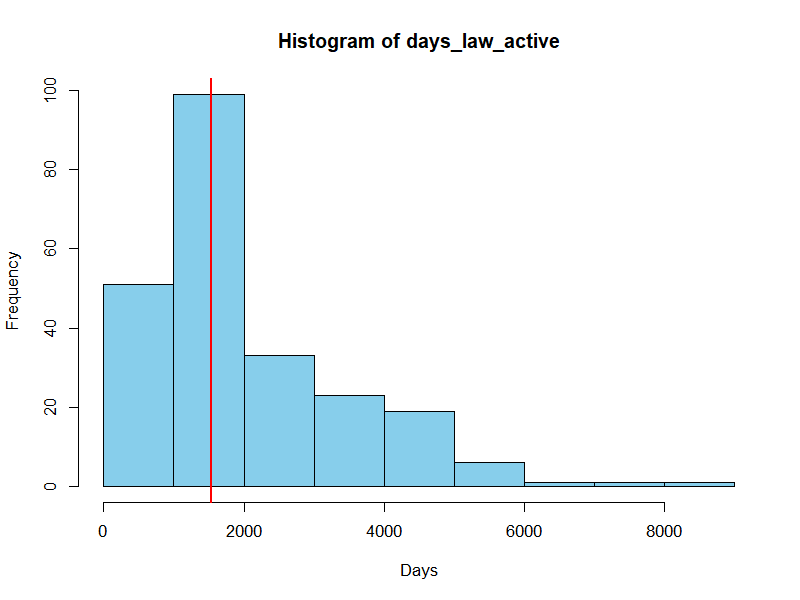
\includegraphics[width=6.25in,height=\textheight]{images/histogram.png}

\hypertarget{finding-1}{%
\subsubsection{Finding 1}\label{finding-1}}

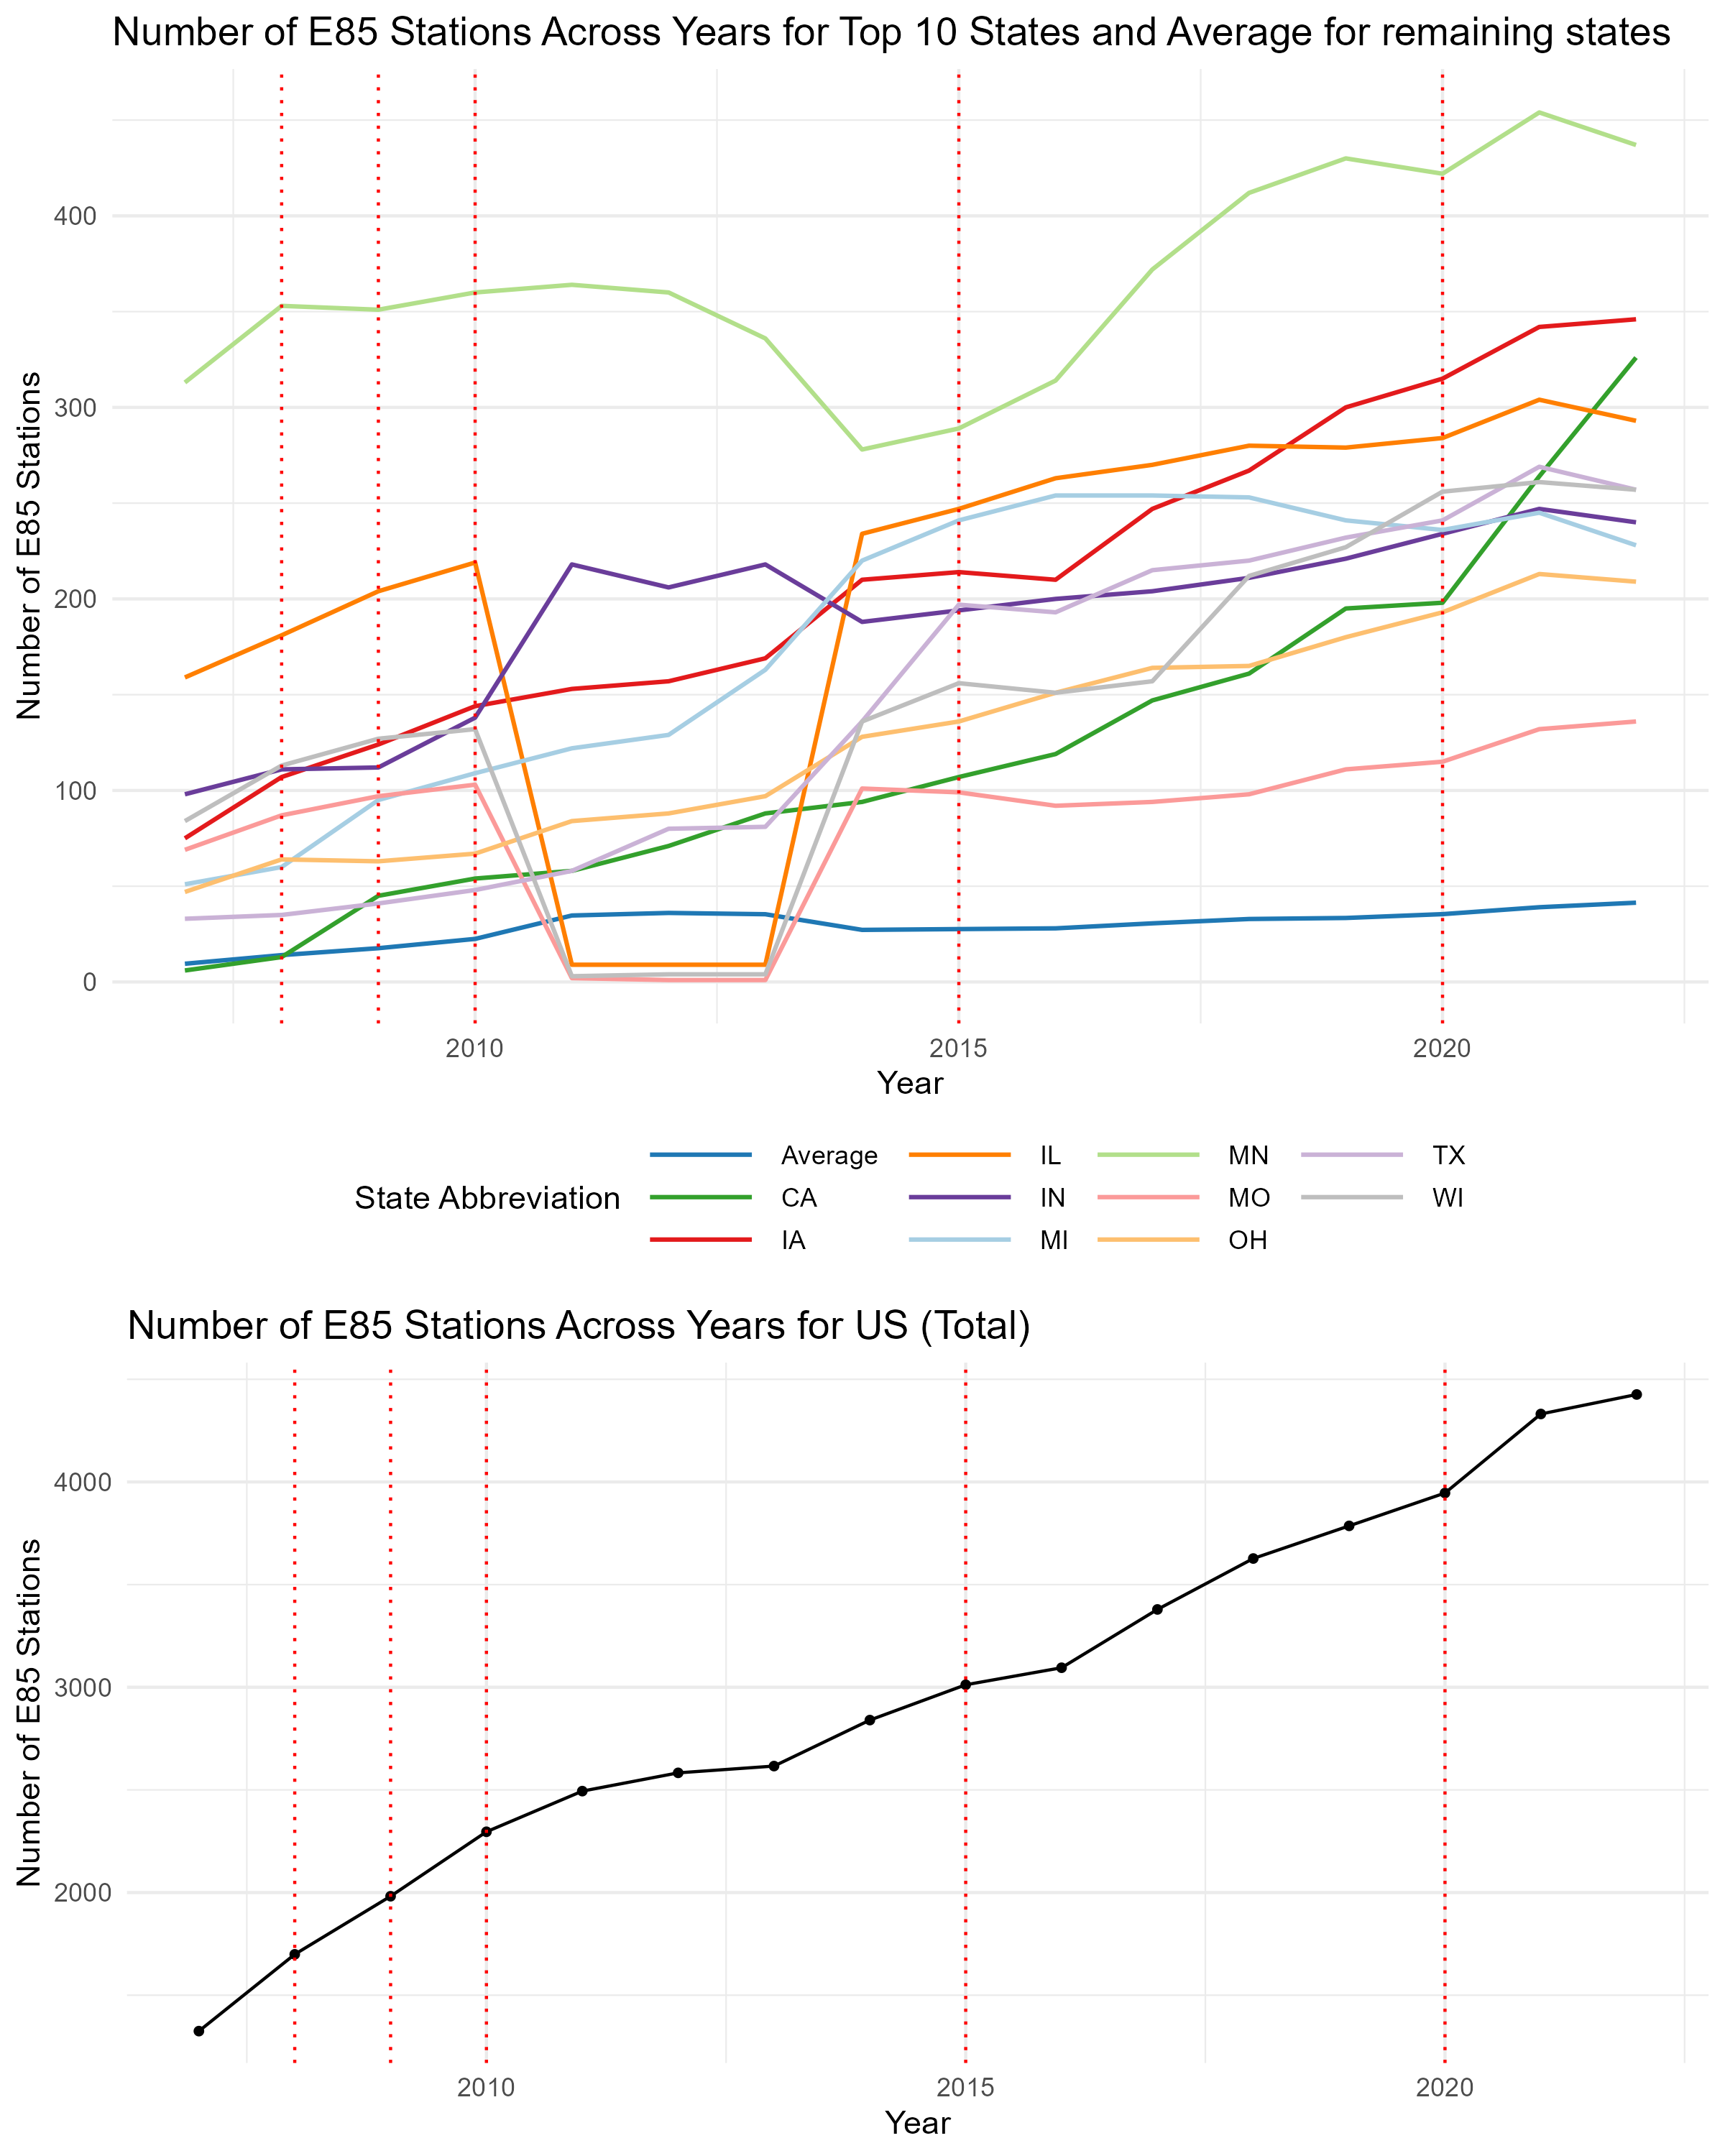
\includegraphics[width=6.25in,height=\textheight]{images/e85_overtime_graph.png}

These first two graphs show the number of E85 stations between 2007 and
2021 for (1) the top 10 states with the highest number of stations as
well as (2) trend in total US E85 gas stations. In the first graph, we
include the average for the remaining states which represent a
proportionally small share of E85 stations as compared to the top ten
states. Dotted vertical lines indicate the enactment of federal-level
laws. We see that the overall number of E85 stations grow over time for
all states with the absolute leader being Minnesota. It is interesting
to note that the number of E85 stations fell down for some states
between 2013 and 2015. Within a span between 2007 and 2021, the total
count of E85 stations in the country more than doubled. Interestingly,
it is apparent that, with the exception of the law implemented in 2020,
it is not obvious that federal-level legislation had an impact across
states on the number of E85 gas stations. Instead, the subsequent rise
in E85 stations was a result of collective growth across all states,
underscoring the influence of aggregate expansion rather than the direct
effect of federal laws.

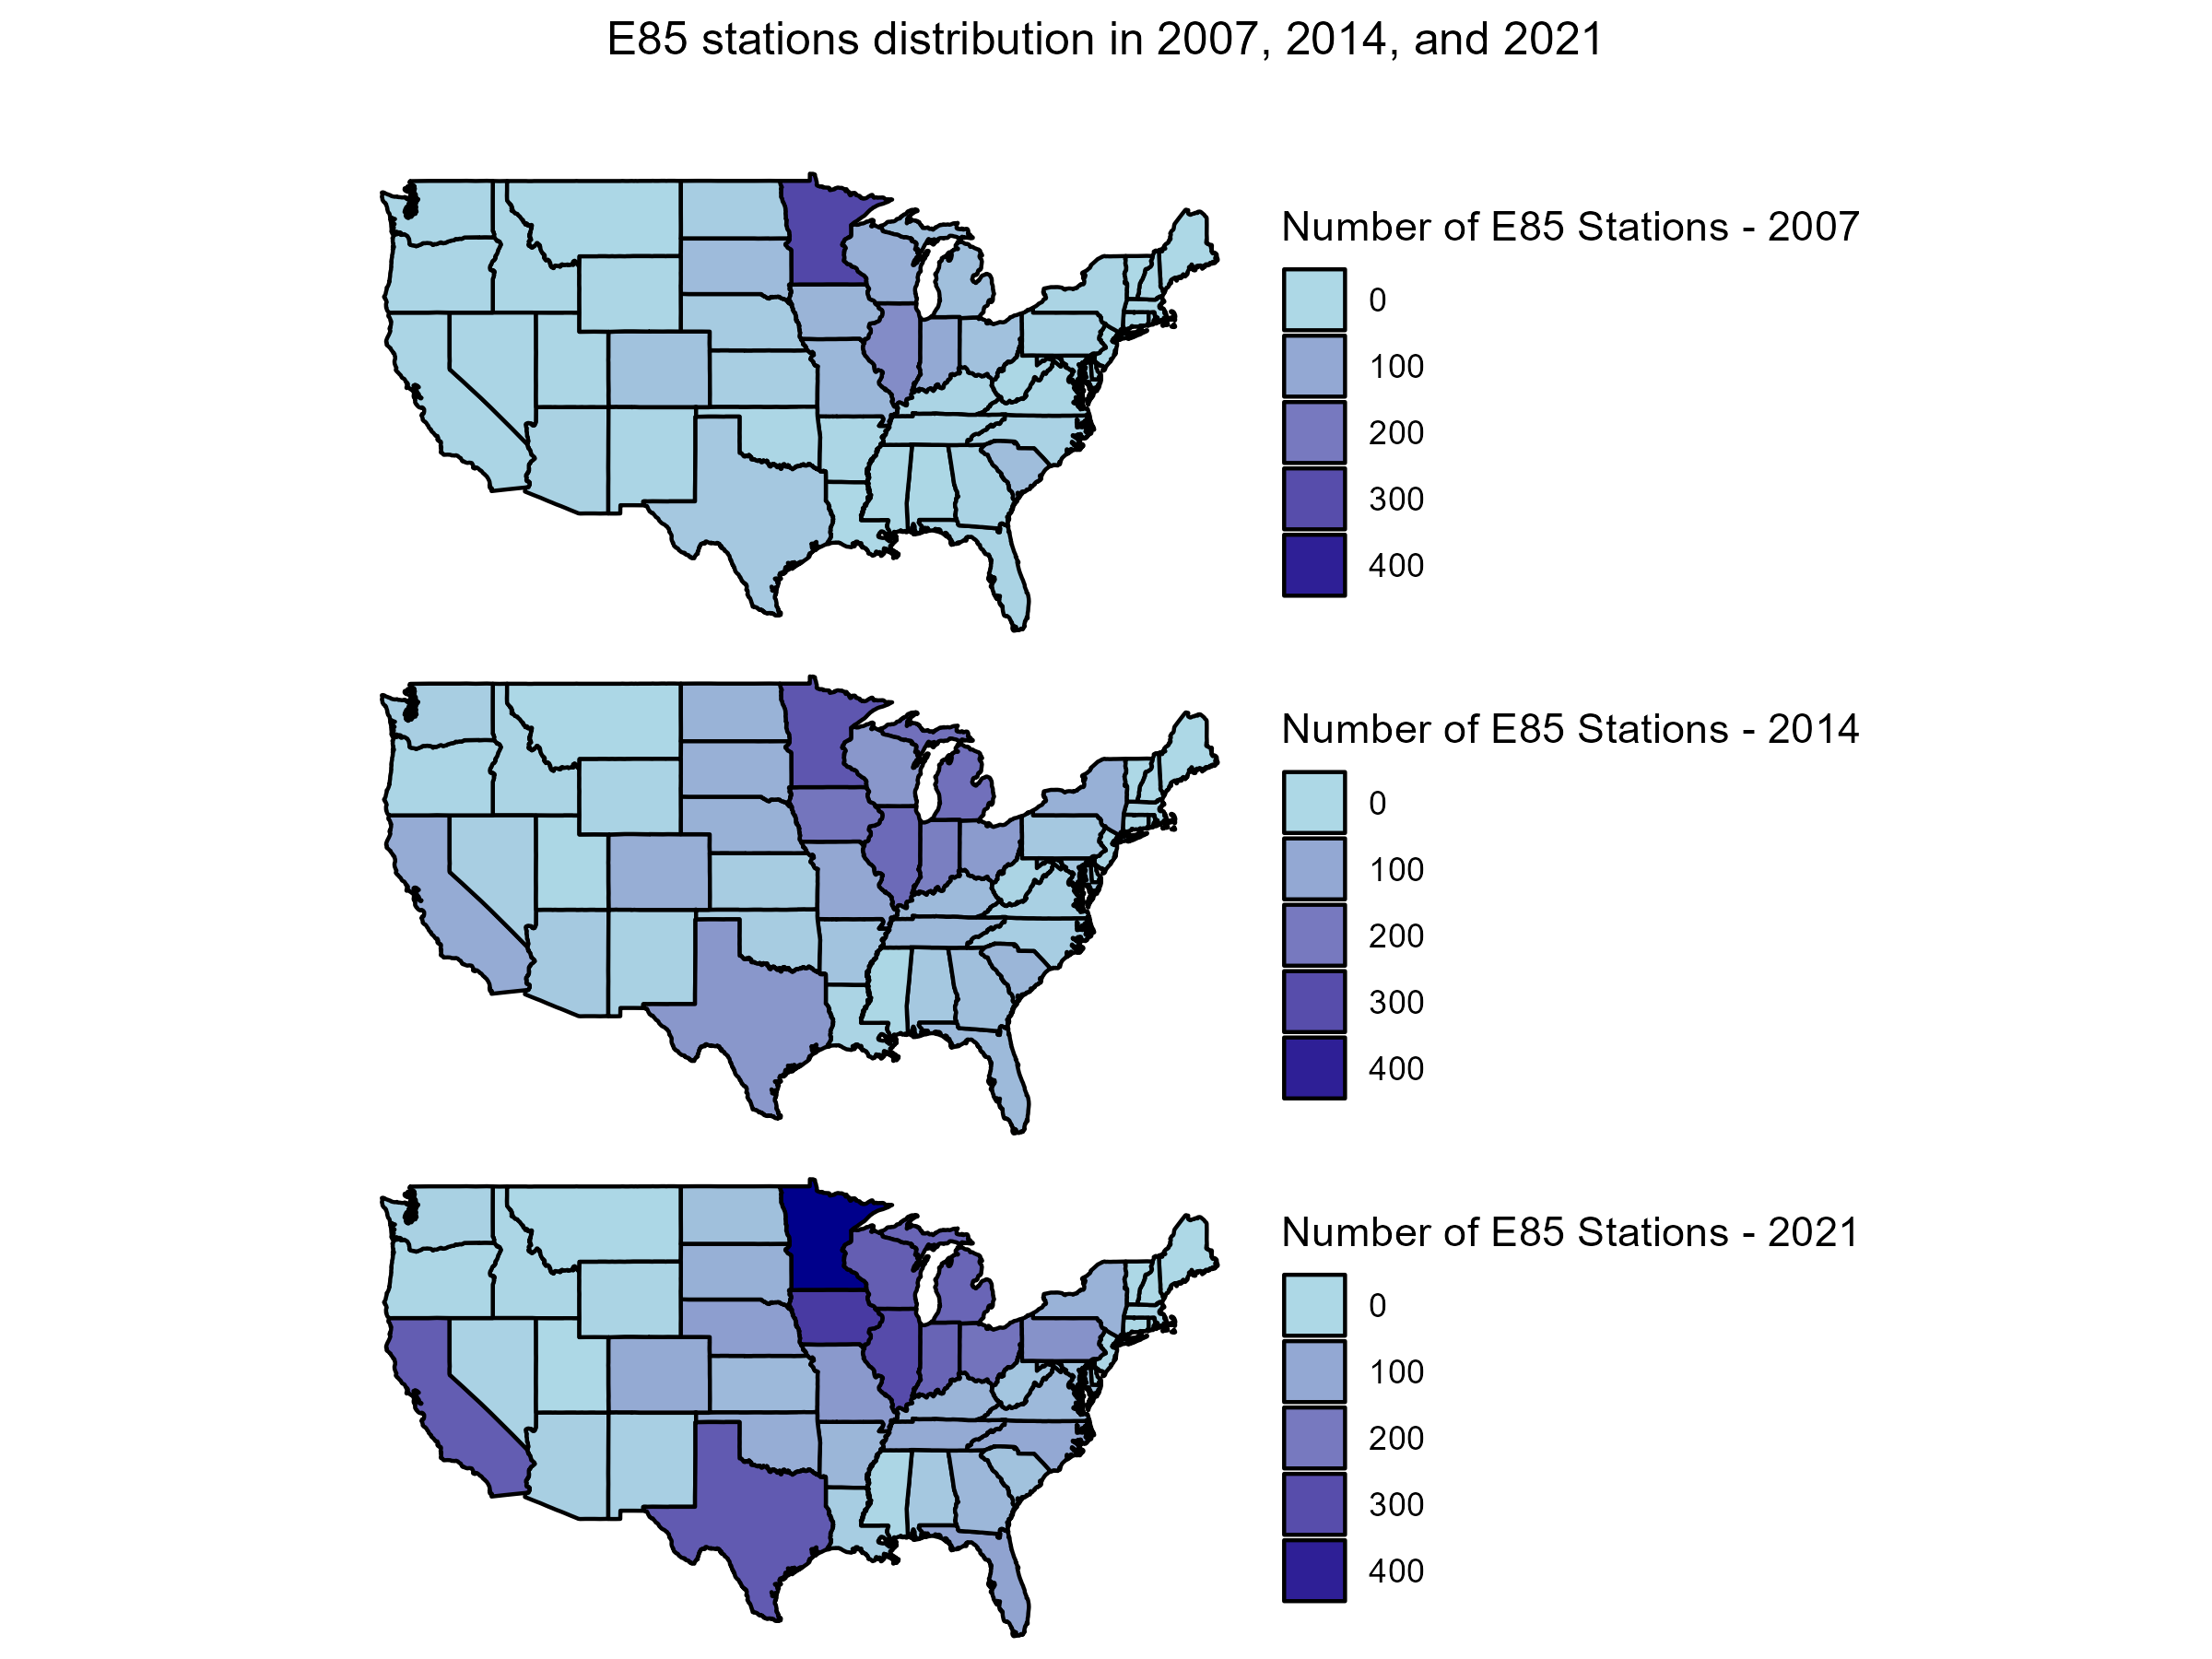
\includegraphics[width=6.25in,height=\textheight]{images/e85_overtime_map-01.png}

This third graphic is composed of three maps showing the distribution of
E85 stations across the US in 2007, 2014 and 2021. The darker shades
correspond to a higher number of E85 stations. We see gradual increase
in E85 station number across states with the corn belt states having the
highest number of E85 along with Texas and California.

\hypertarget{finding-2}{%
\subsubsection{Finding 2}\label{finding-2}}

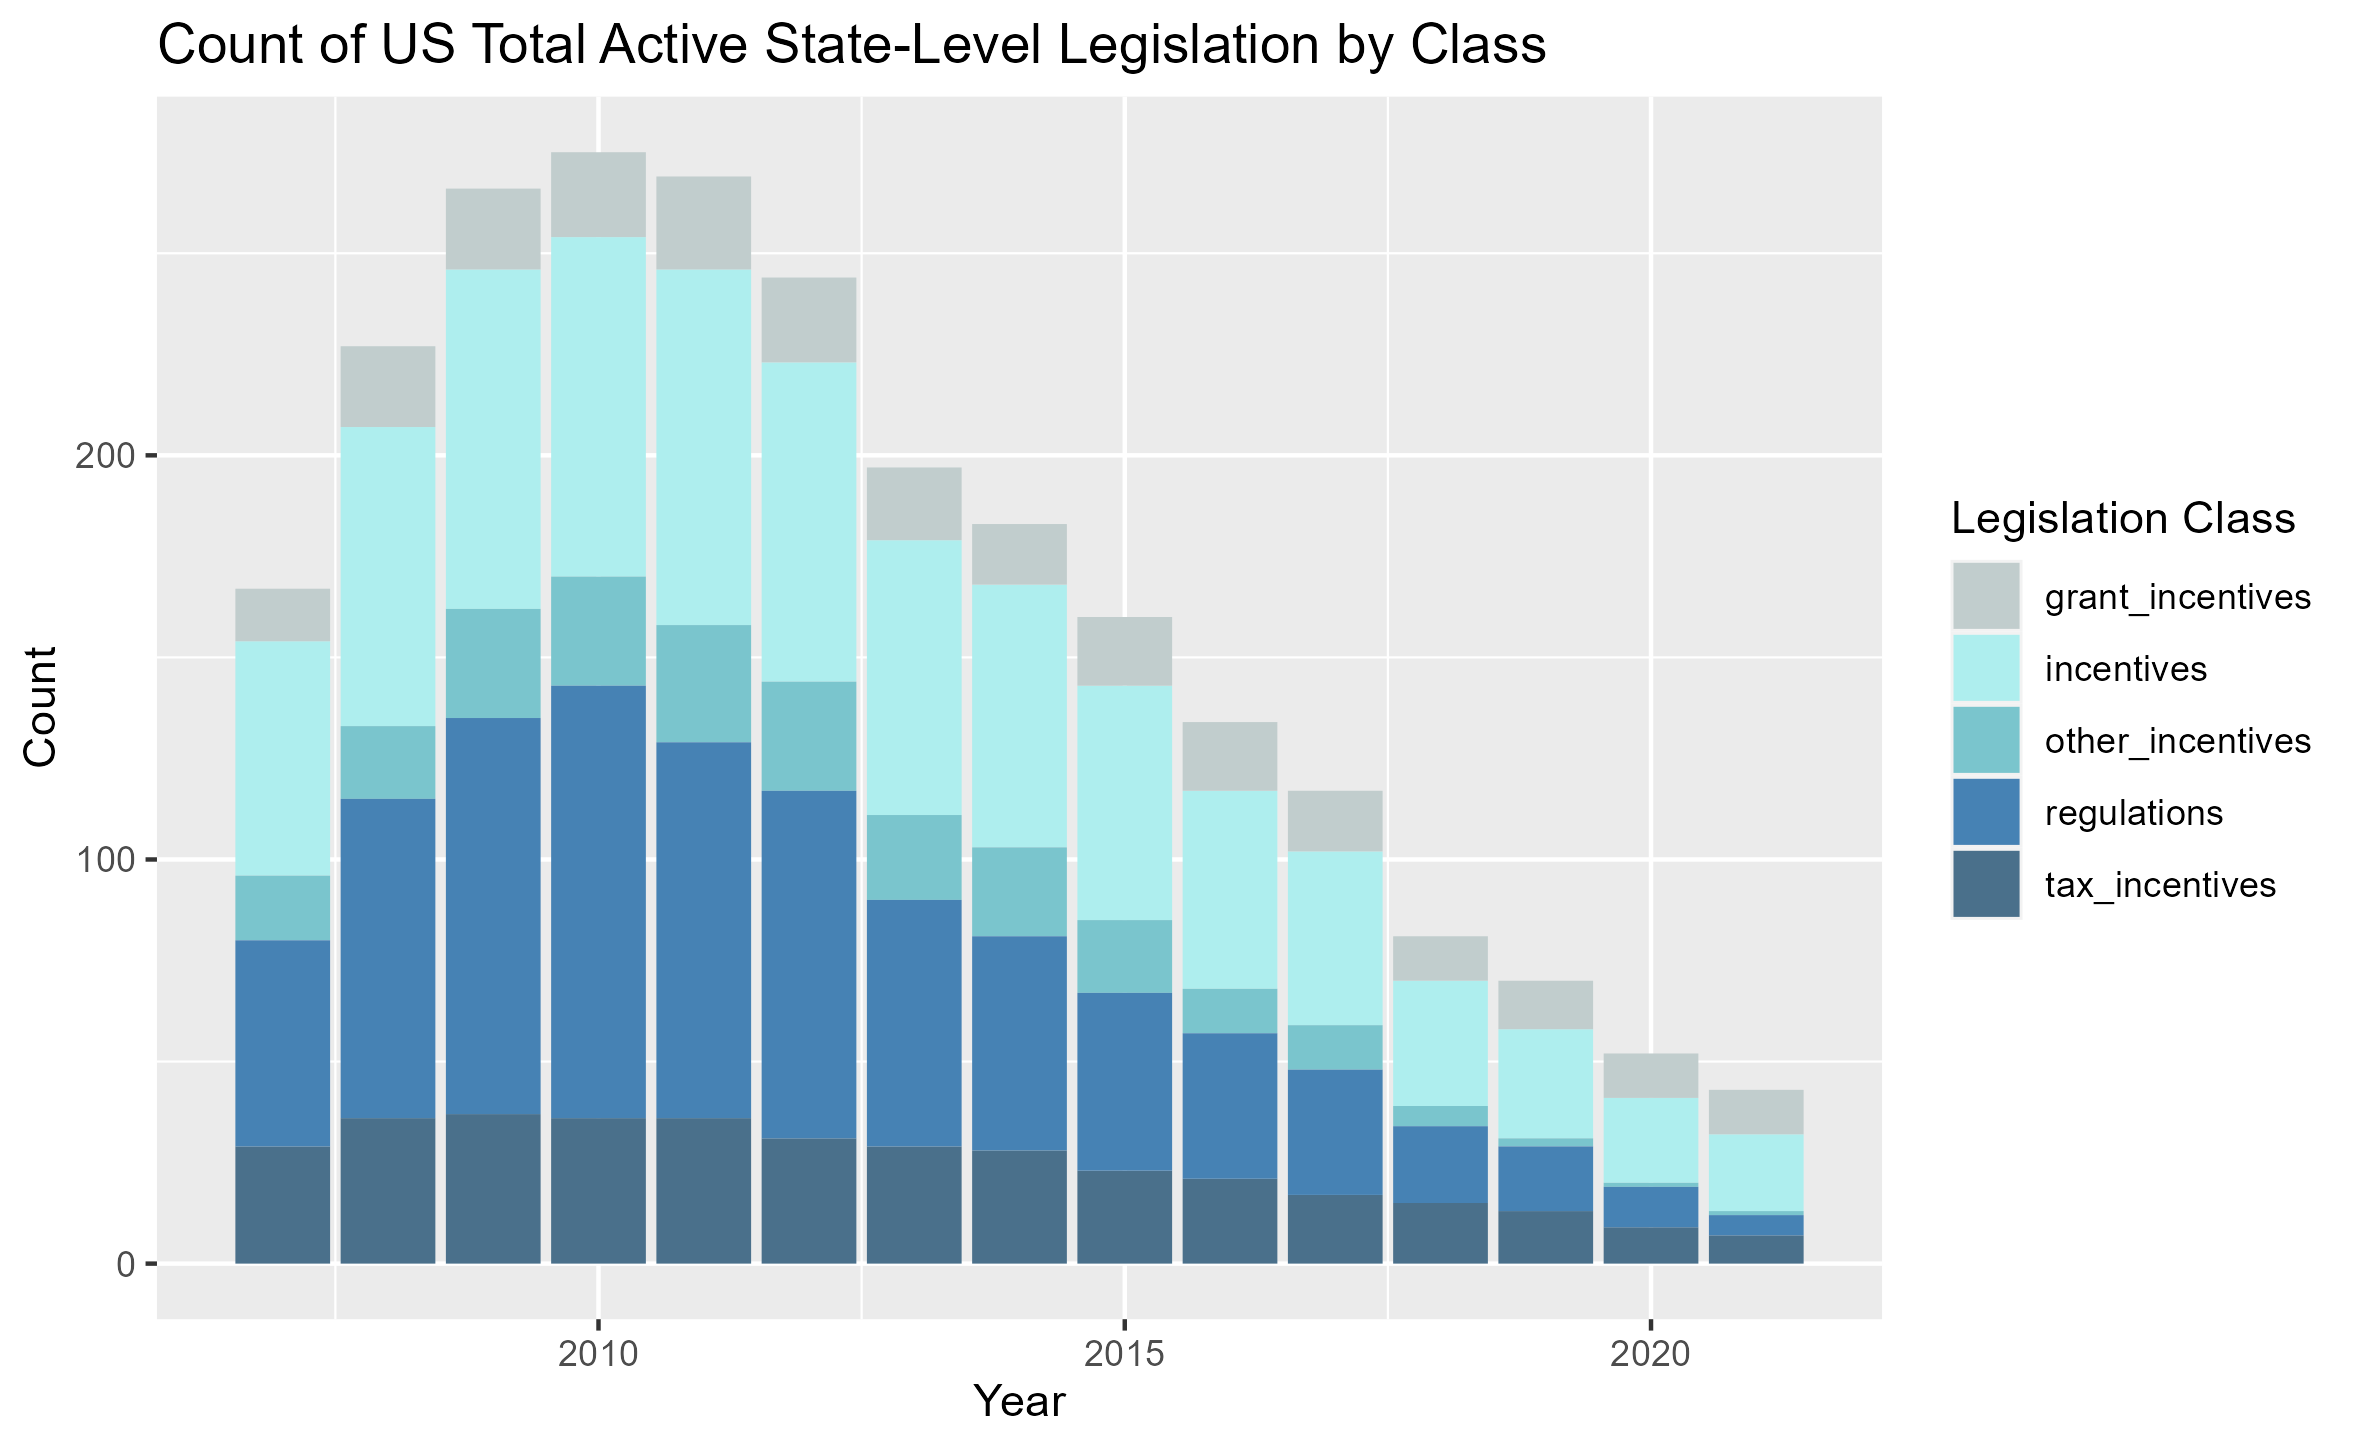
\includegraphics[width=6.25in,height=\textheight]{images/StackedTotalLeg.png}

Through this graph, we can see that at the beginning of our time period
of interest, there was a significant increase in active legislation
relating to ethanol. Today, most of that legislation has been repealed
or is no longer active. This allows us to infer two things. First,
ethanol-related legislation in the form of grants or incentives may have
allowed for capital investments in ethanol production and distribution
which would have effects on the number of E85 stations and ethanol
demand. The effects of this legislation may still persist while the
actual legislation has expired or been repealed because improvements to
capital infrastructure do not necessarily need to be perpetual.
Secondly, there may be a reduction in ethanol related legislation
because the legislation was repealed due to it no longer being valued or
because it was considered ineffective. This would imply that the
legislation had no impact on the number of E85 stations and,
subsequently, demand.

\hypertarget{finding-3}{%
\subsubsection{Finding 3}\label{finding-3}}

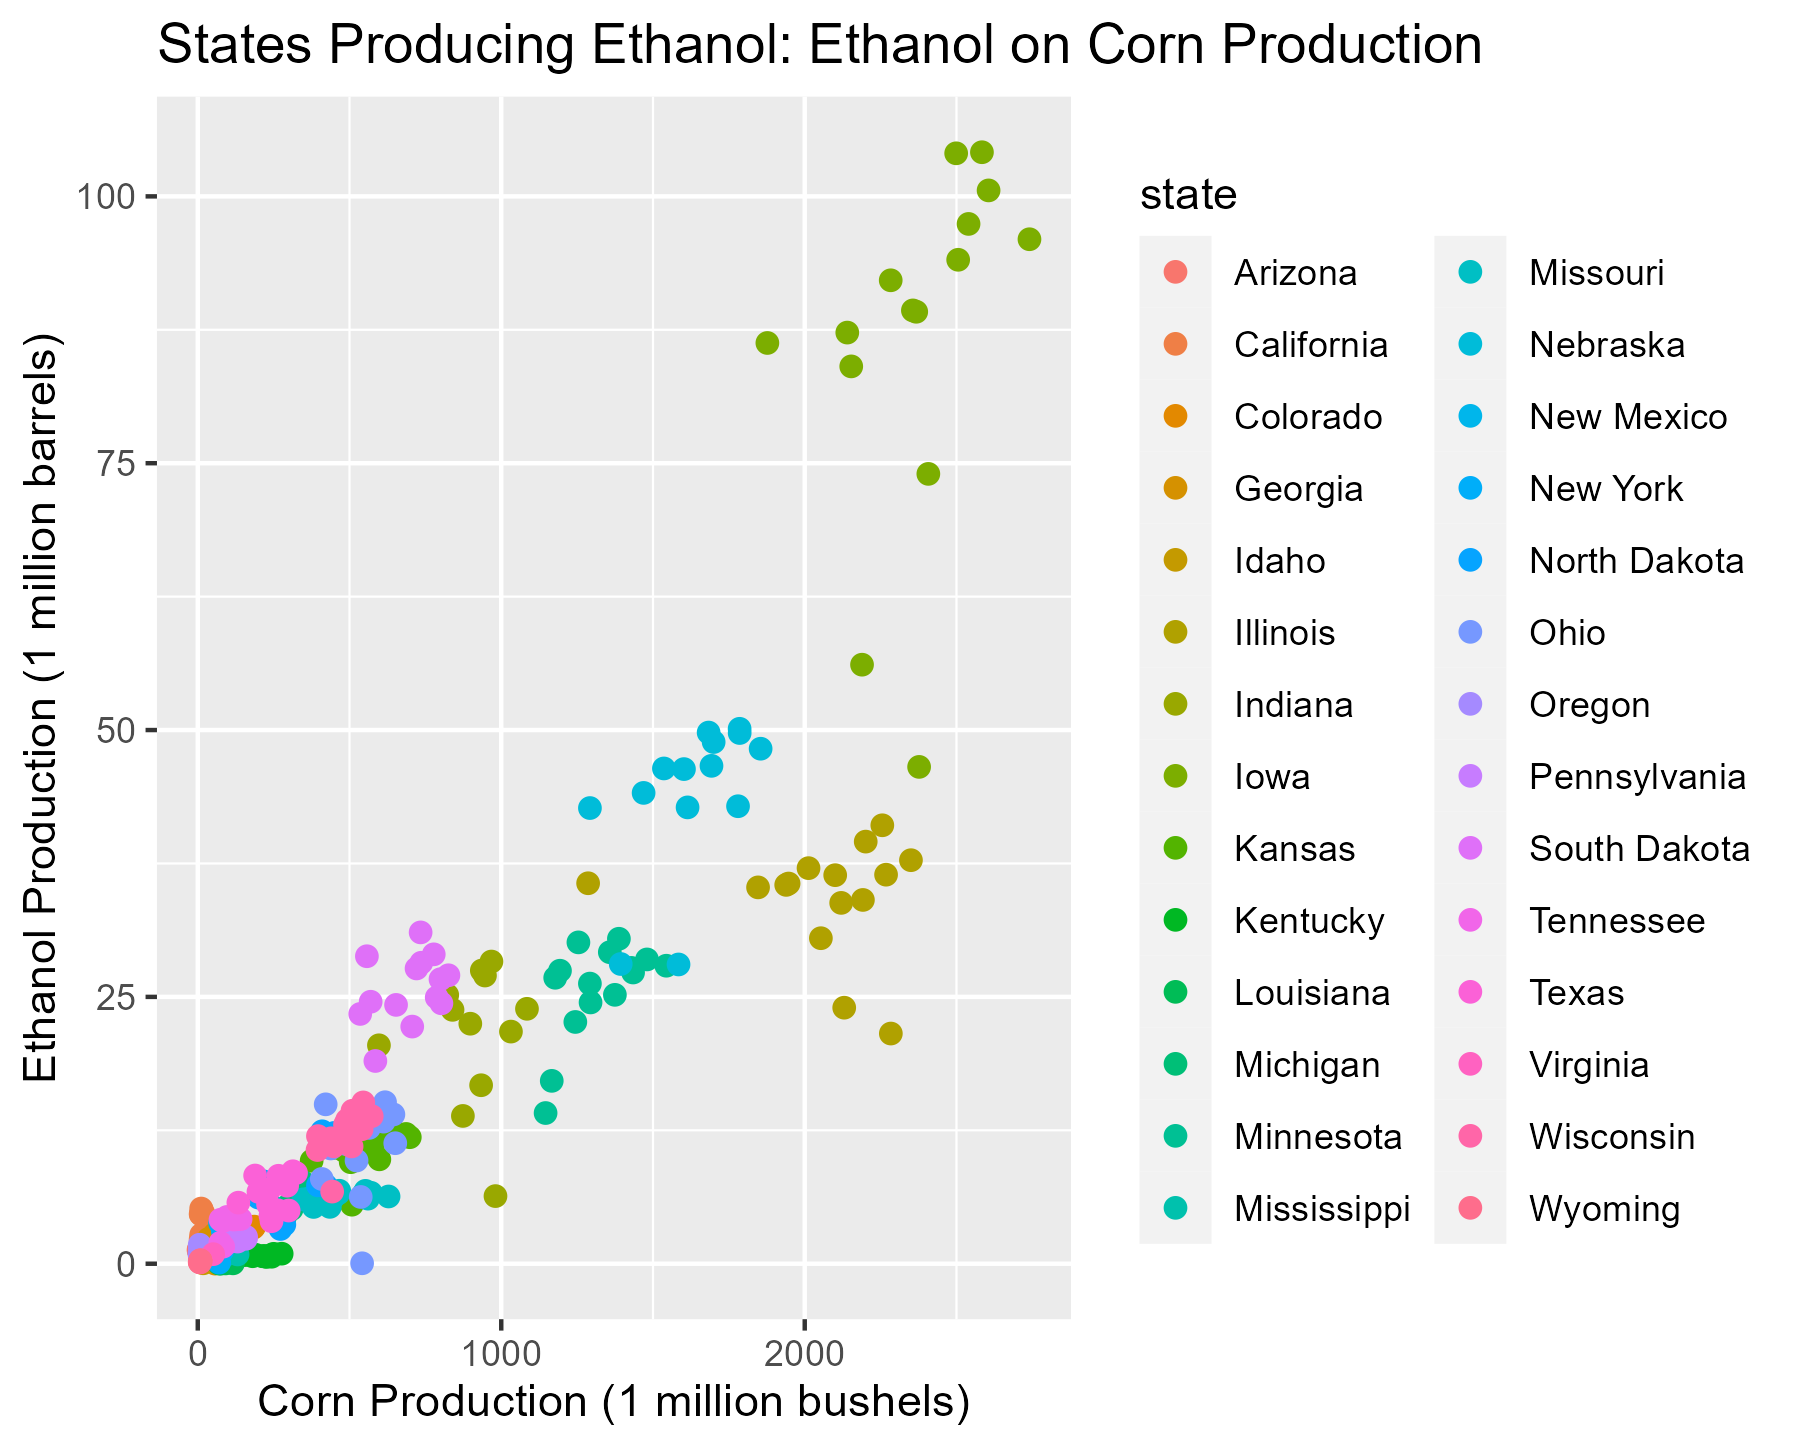
\includegraphics[width=6.25in,height=\textheight]{images/EthCornScatterByState.png}

Ethanol production is clearly higher in states which have larger corn
production. States with high corn and ethanol production include Iowa,
Missouri, and Illinois. This implies that much of the ethanol produced
in the United States is produced in states which also produce a lot of
corn - likely due to market effects incentivizing minimization of
transportation costs. Corn production and ethanol production is not
particularly variable across years (each data point represents ethanol
and corn production for a state in a given year). One of the things we
can infer from this is that capital investments are large enough to
require supply of ethanol and corn production to be relatively stable.

\hypertarget{finding-4}{%
\subsubsection{Finding 4}\label{finding-4}}

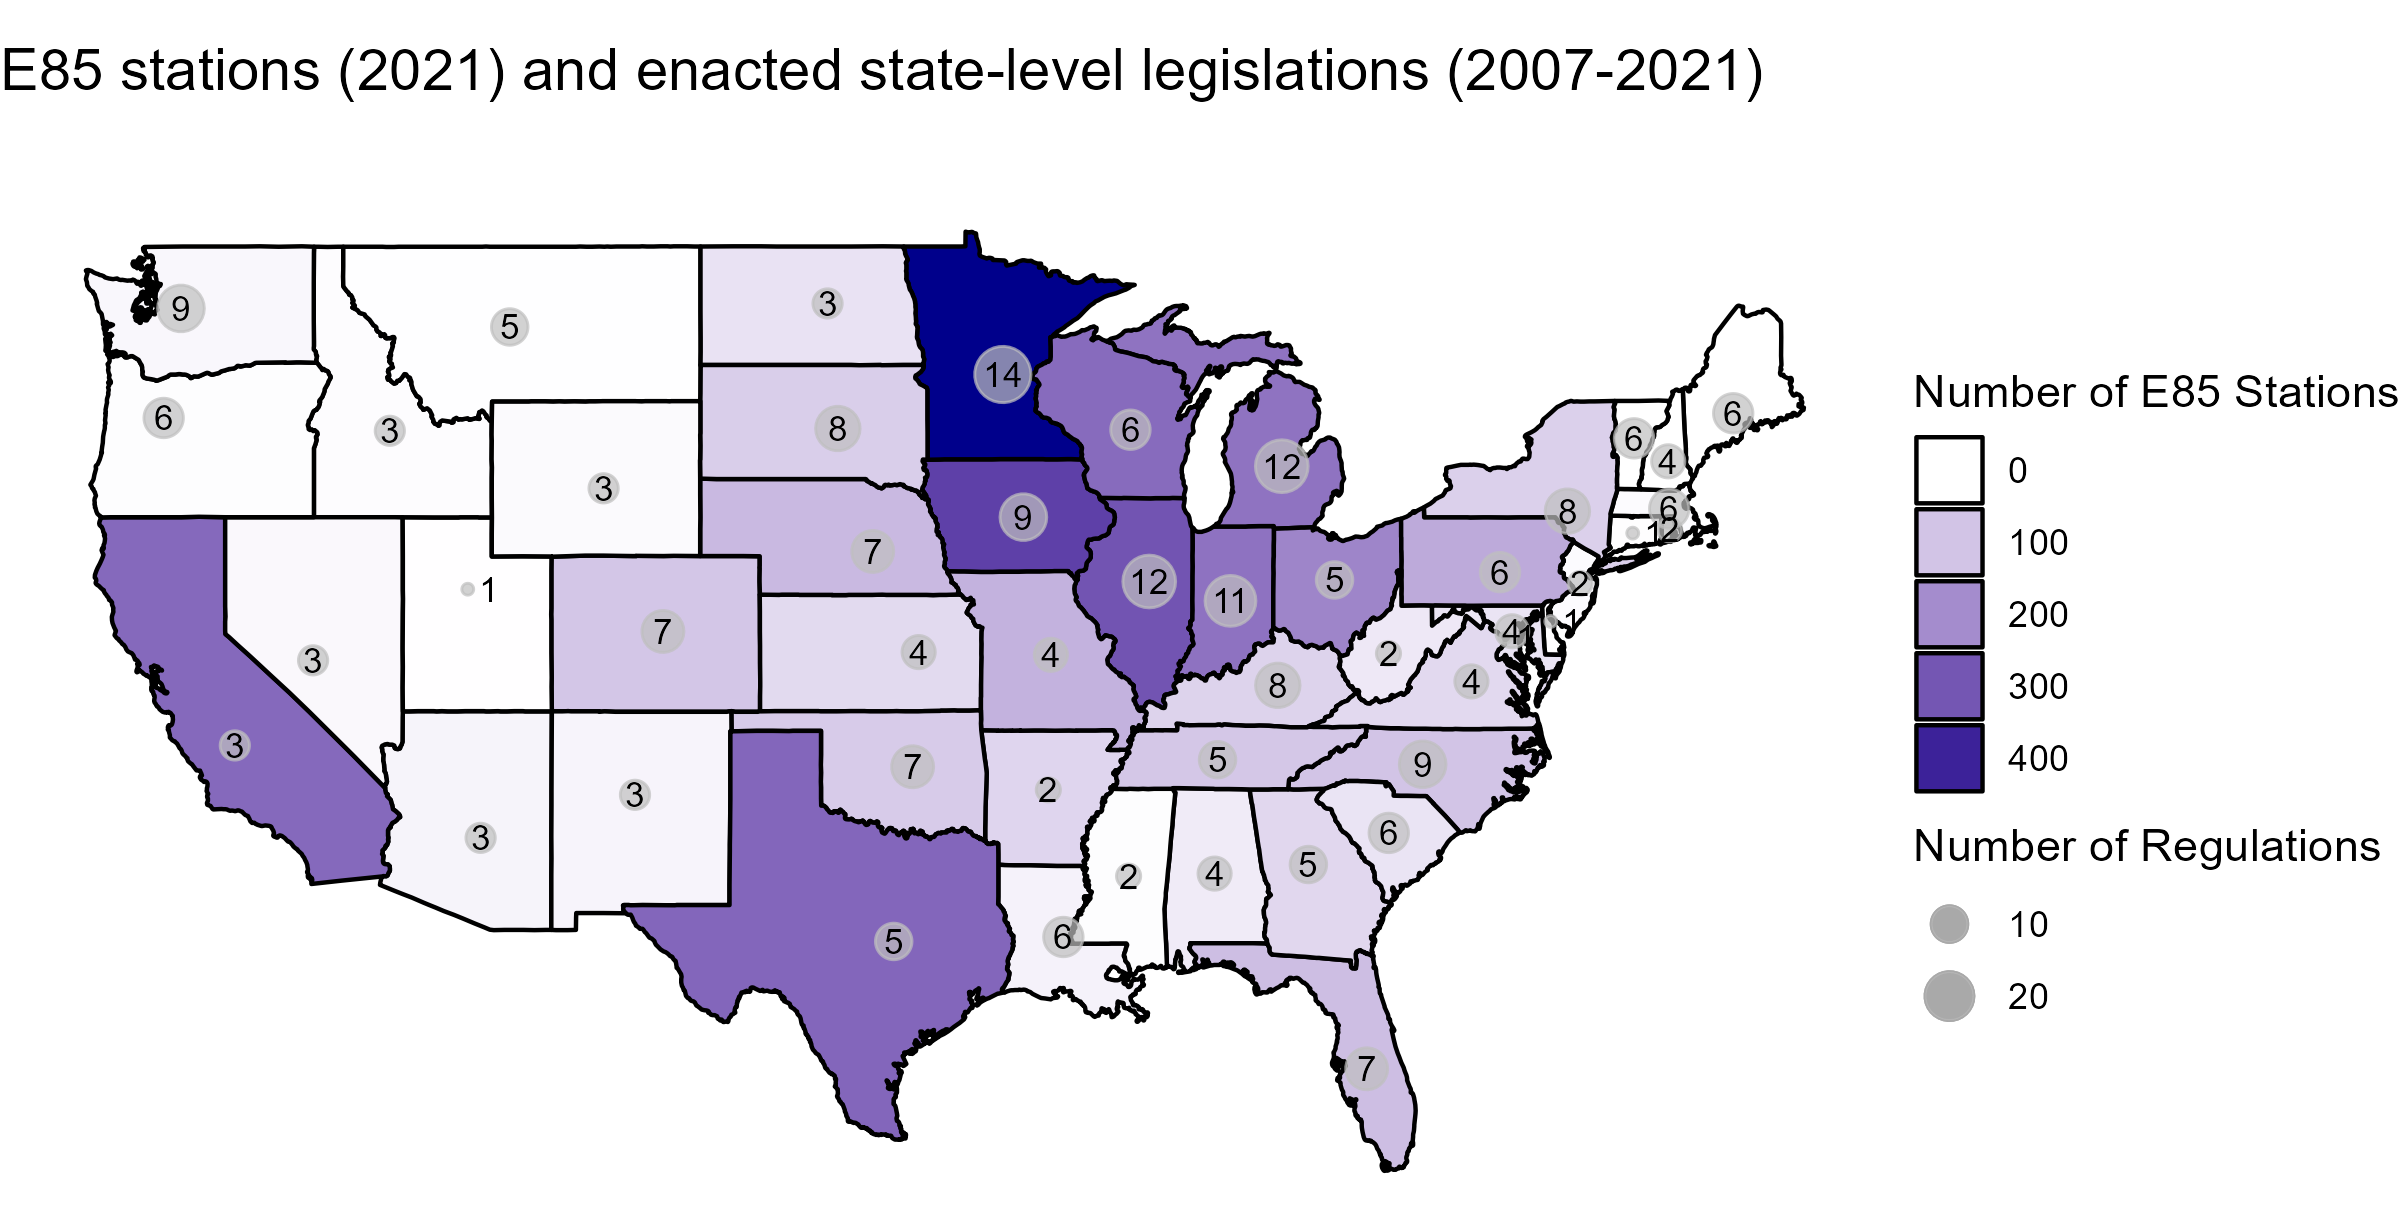
\includegraphics[width=6.25in,height=\textheight]{images/e85_legislations_map-04.png}

This first map illustrates the distribution of E85 stations across the
US in 2021, with gray dots representing the number of laws enacted
between 2007 and 2021 in each state. Larger dots indicate a higher
number of legislations, while darker shades signify a greater number of
E85 stations. The pattern reveals that states with fewer legislations
(ranging from 0 to 2) tend to have fewer E85 stations. However, the
relationship becomes less clear in states with higher numbers of
incentives and regulations. For instance, both Nevada and California
have enacted 3 legislations, yet the number of E85 stations in these
states varies significantly.
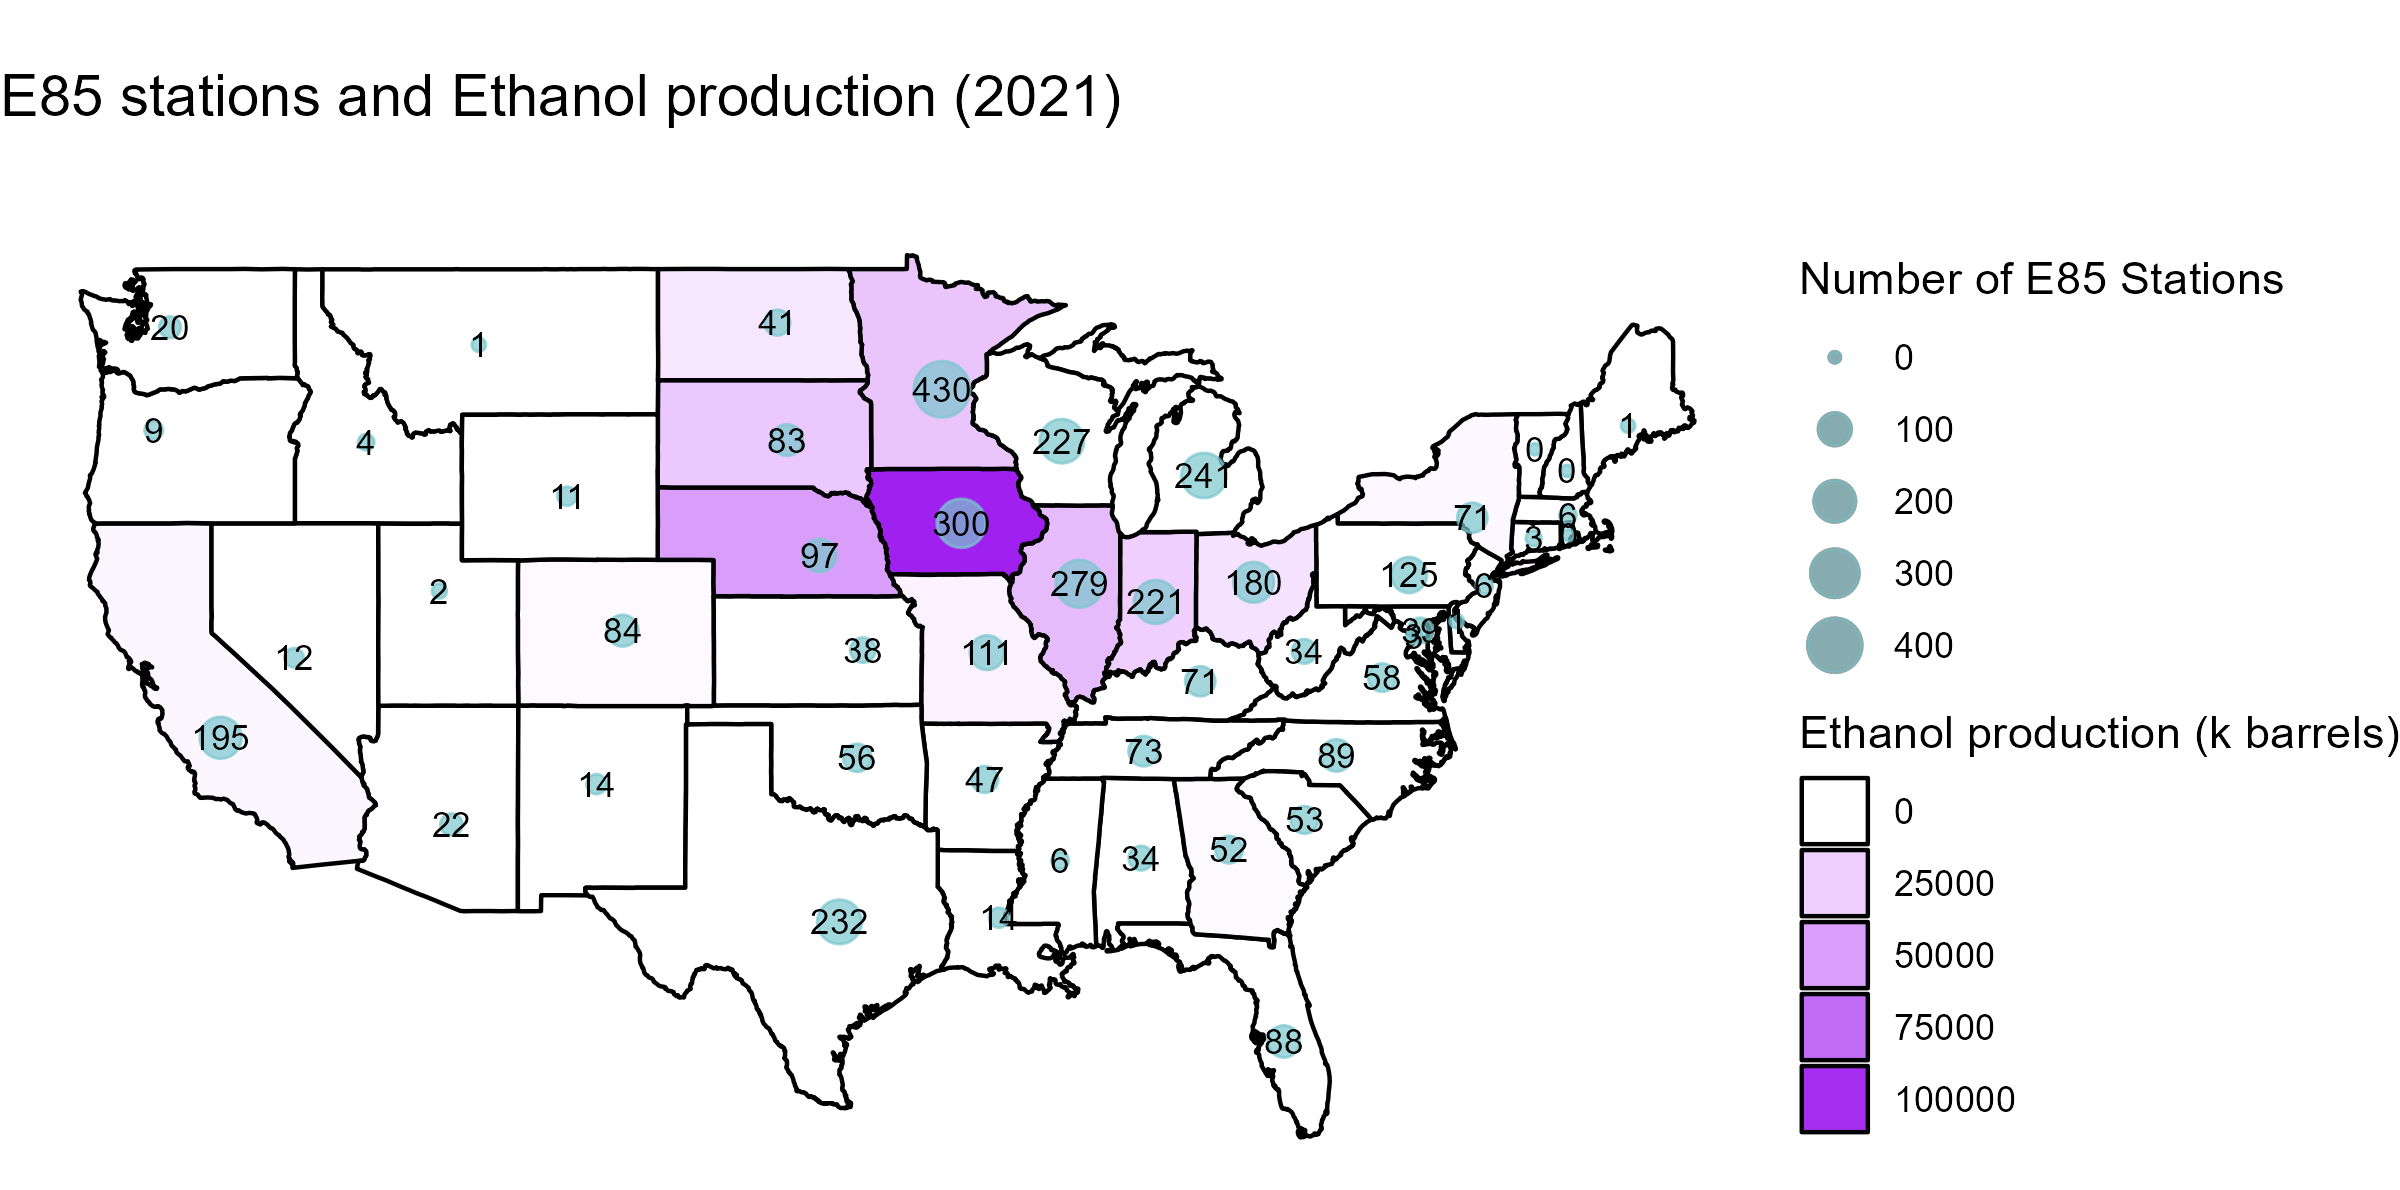
\includegraphics[width=6.25in,height=\textheight]{images/ethanol_production_e85.png}

This second map illustrates distribution of ethanol production across
the US in 2021 with blue dots representing the number of E85 stations
available in each state in 2021. Larger dots indicate a higher number of
E85 stations, while darker shades signify a greater amount of ethanol
produced. We do not see a clear relationship between the number of E85
stations and ethanol produced with high producing states like Iowa and
Illinois having significantly different numbers of E85 stations
available.

\hypertarget{finding-5}{%
\subsubsection{Finding 5}\label{finding-5}}

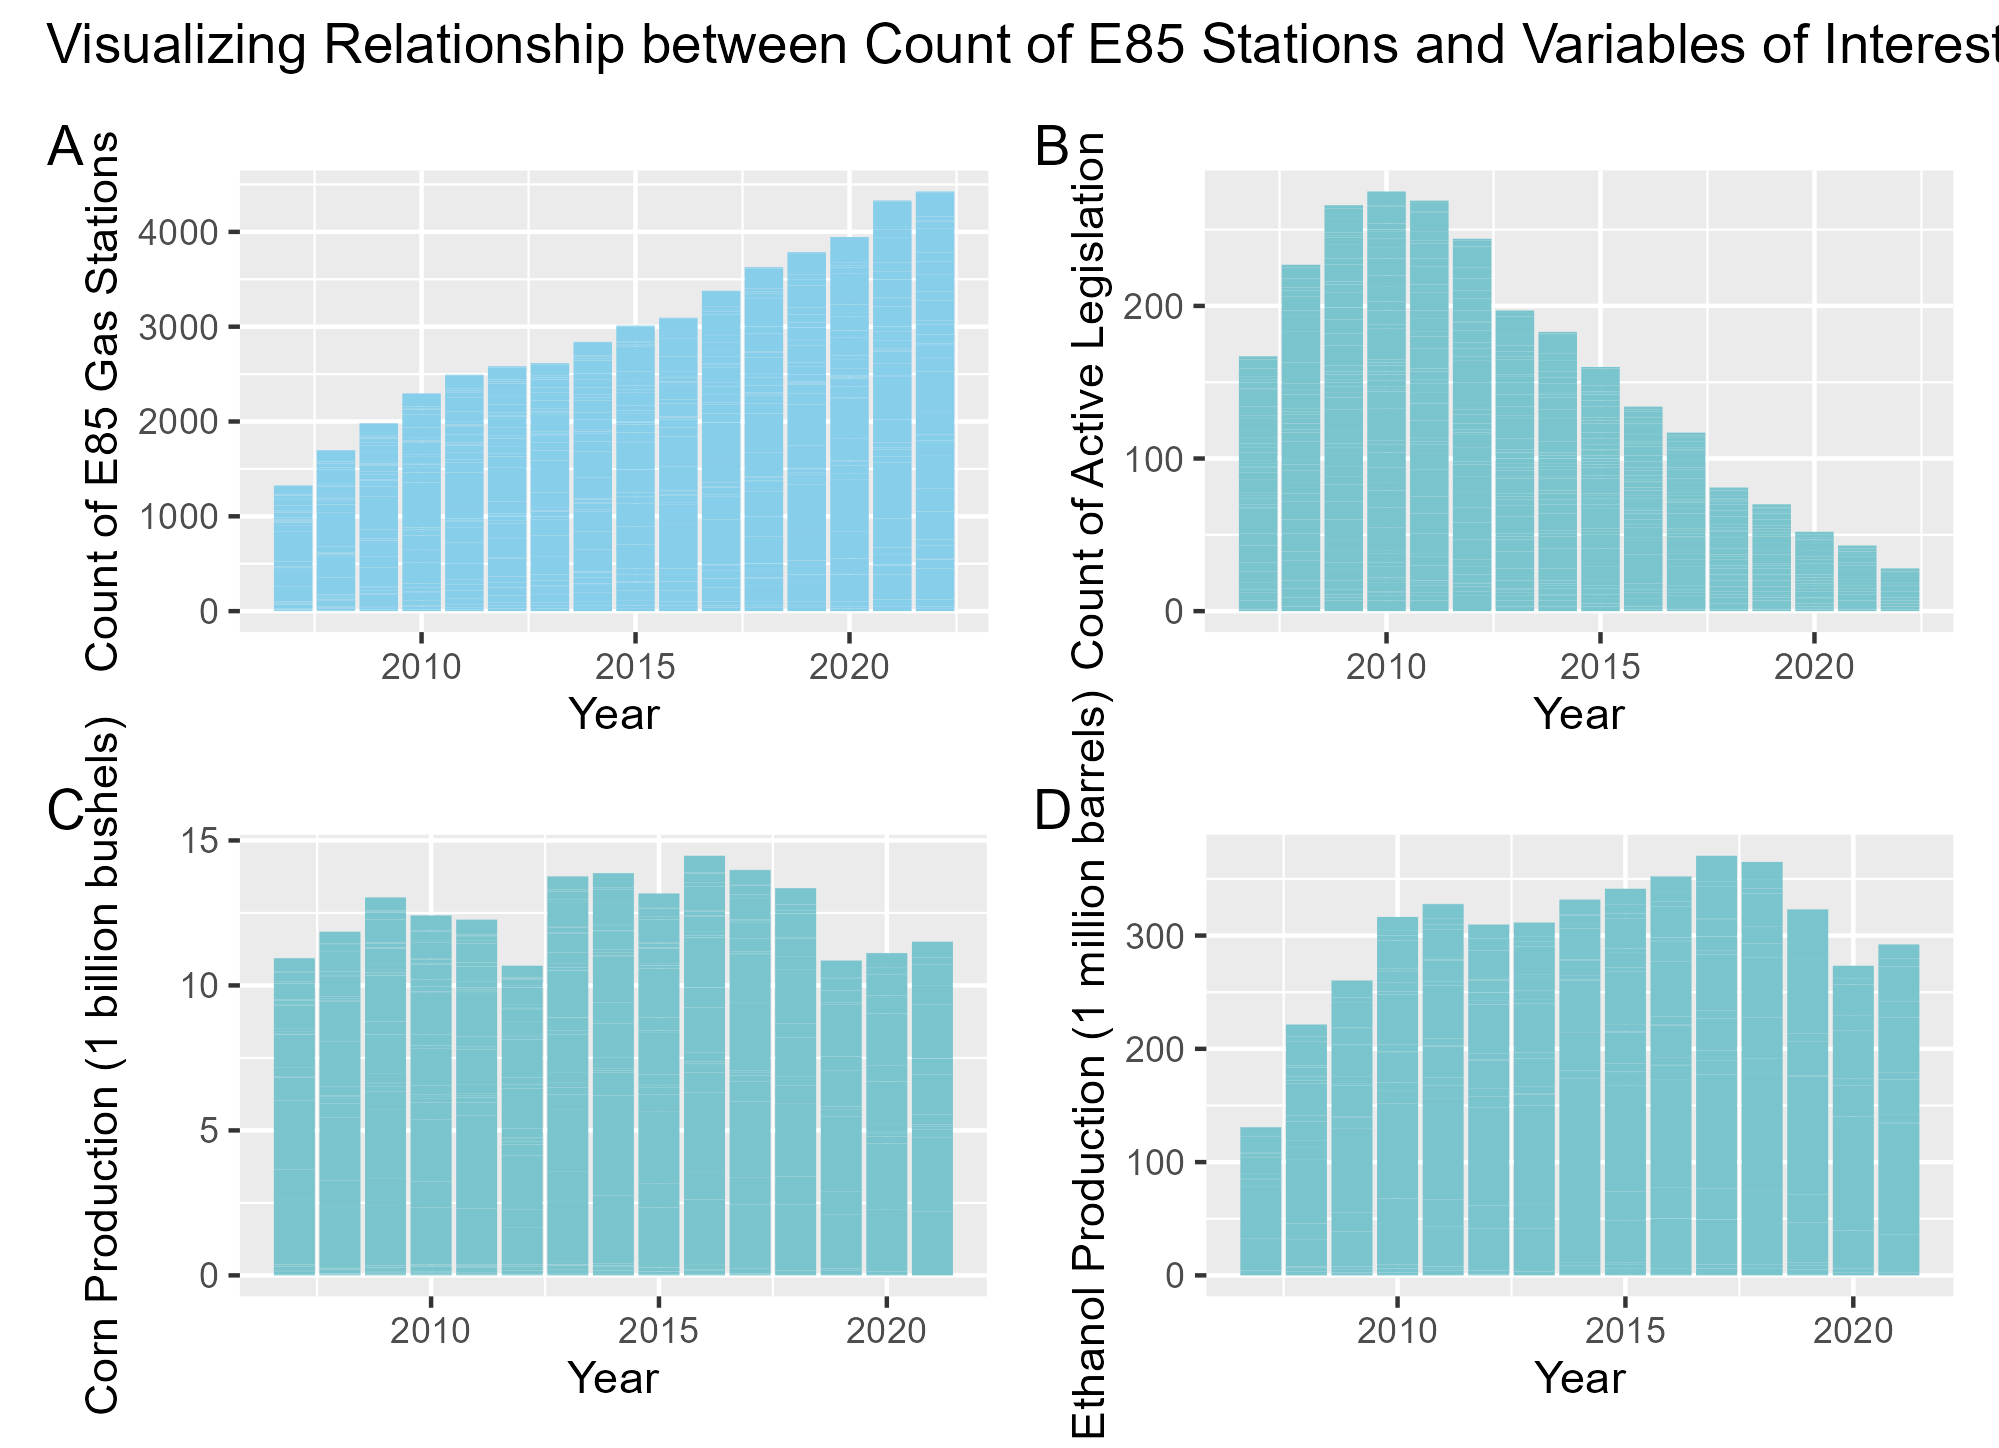
\includegraphics[width=6.25in,height=\textheight]{images/E85Relationships.png}

Through this graphic, we are able to identify that the total number of
E85 gas stations in the United States increased following significant
increases in the number of active state-level legislation in the United
States. We can see that corn production does not vary significantly
(ethanol related legislation is likely not affecting the amount of corn
produced), but ethanol production does increase as active ethanol
related legislation increases. Ethanol related legislation is associated
with increases in ethanol production and E85 demand implying that
legislation helped bolster the market for ethanol.

\end{document}
